
%(BEGIN_QUESTION)
% Copyright 2015, Tony R. Kuphaldt, released under the Creative Commons Attribution License (v 1.0)
% This means you may do almost anything with this work of mine, so long as you give me proper credit

\noindent
{\bf Lab Exercise -- introduction}

\vskip 5pt

Your team's task is to commission and test a protective relay for one protection zone within the lab's miniature three-phase power grid.  Your instructor will assign a protection zone for your team.

The following table of objectives show what you and your team must complete within the scheduled time for this lab exercise.  Note how some of these objectives are individual, while others are for the team as a whole:

\underbar{Objective completion table:}

% No blank lines allowed between lines of an \halign structure!
% I use comments (%) instead, so that TeX doesn't choke.

$$\vbox{\offinterlineskip
\halign{\strut
\vrule \quad\hfil # \ \hfil & 
\vrule \quad\hfil # \ \hfil & 
\vrule \quad\hfil # \ \hfil & 
\vrule \quad\hfil # \ \hfil & 
\vrule \quad\hfil # \ \hfil & 
\vrule \quad\hfil # \ \hfil & 
\vrule \quad\hfil # \ \hfil \vrule \cr
\noalign{\hrule}
%
% First row
{\bf Performance objective} & {\bf Grading} & {\bf 1} & {\bf 2} & {\bf 3} & {\bf 4} & {\bf Team} \cr
%
\noalign{\hrule}
%
% Another row
Team meeting & mastery & -- & -- & -- & -- & \cr
%
\noalign{\hrule}
%
% Another row
Verify phase rotation of a three-phase source & mastery & -- & -- & -- & -- &  \cr
%
\noalign{\hrule}
%
% Another row
Commissioning tests and system inspection & mastery & -- & -- & -- & -- &  \cr
%
\noalign{\hrule}
%
% Another row
Test e/m 50 (inst. overcurrent) relay & mastery & -- & -- & -- & -- &  \cr
%
\noalign{\hrule}
%
% Another row
Test e/m 51 (time overcurrent) relay & mastery & -- & -- & -- & -- &  \cr
%
\noalign{\hrule}
%
% Another row
``Stab'' into a live CT circuit to measure current & mastery & & & & & -- -- -- -- \cr
%
\noalign{\hrule}
%
% Another row
Manually synchronize a generator with the grid & mastery & & & & & -- -- -- -- \cr
%
\noalign{\hrule}
%
% Another row
Configure digital relay per specification & mastery & & & & & -- -- -- -- \cr
%
\noalign{\hrule}
%
% Another row
Simulated fault and relay event report & mastery & -- & -- & -- & -- &  \cr
%
\noalign{\hrule}
%
% Another row
Lab question: Wiring connections & proportional &  &  &  &  & -- -- -- -- \cr
%
\noalign{\hrule}
%
% Another row
Lab question: Commissioning & proportional &  &  &  &  & -- -- -- -- \cr
%
\noalign{\hrule}
%
% Another row
Lab question: Mental math & proportional &  &  &  &  & -- -- -- -- \cr
%
\noalign{\hrule}
%
% Another row
Lab question: Diagnostics & proportional &  &  &  &  & -- -- -- -- \cr
%
\noalign{\hrule}
%
% Another row
Lab clean-up & mastery & -- & -- & -- & -- &  \cr
%
\noalign{\hrule}
} % End of \halign 
}$$ % End of \vbox

The only ``proportional'' scoring in this activity are the lab questions, which are answered by each student individually.  A listing of potential lab questions are shown at the end of this worksheet question.  The lab questions are intended to guide your labwork as much as they are intended to measure your comprehension, and as such the instructor may ask these questions of your team day by day, rather than all at once (on a single day).

{\bf It is essential that your team plans ahead what to accomplish each day.  A short (10 minute) team meeting at the beginning of each lab session is a good way to do this, reviewing what's already been done, what's left to do, and what assessments you should be ready for.  There is a lot of work involved with building, documenting, and troubleshooting these working instrument systems!}

As you and your team work on this system, you will invariably encounter problems.  You should always attempt to solve these problems as a team before requesting instructor assistance.  If you still require instructor assistance, write your team's color on the lab whiteboard with a brief description of what you need help on.  The instructor will meet with each team in order they appear on the whiteboard to address these problems.





\vfil \eject

\noindent
{\bf Lab Exercise -- team meeting}

\vskip 5pt

An important first step in completing this lab exercise is to {\bf meet with your instructor} as a team to discuss safety concerns, team performance, and specific roles for team members.  If you would like to emphasize exposure to certain equipment (e.g. use a particular type of control system, certain power tools), techniques (e.g. fabrication), or tasks to improve your skill set, this is the time to make requests of your team so that your learning during this project will be maximized.

\vskip 20pt





%\vfil \eject

\noindent
{\bf Lab Exercise -- phase rotation (sequence) testing}

\vskip 5pt

Once live three-phase power is available in the lab power grid, you will be required to verify its {\it phase rotation} by connecting a suitable test instrument to it, either directly to the power lines (where applicable) or through potential transformers pre-connected to the grid.  If your station happens to be a generator, you will need to verify its phase rotation {\it before} attempting to place it on-line (i.e. close the breaker to connect it to the grid).

\vskip 10pt

Suitable test equipment exists in the lab for you to measure phase rotation.  A multi-channel oscilloscope is one form of suitable test equipment, but others exist as well.  Be sure to consult the manual before using this equipment on the power system, as system voltages and currents are capable of damaging equipment if incorrectly connected.  A sample schematic shown here illustrates how you may build a three-phase voltage divider resistor network to create a three-phase voltage divider for safely testing phase rotation in cases where the line voltage could damage the test instrument's inputs.  This Wye-connected resistor network also provides a ``ground'' reference if the power system lacks one:

$$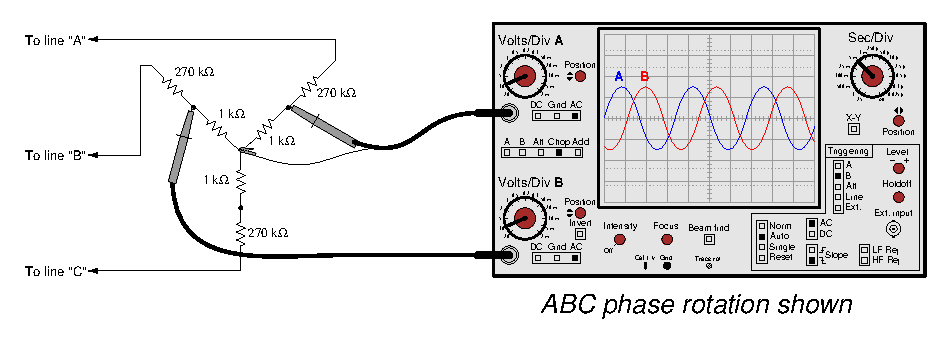
\includegraphics[width=15.5cm]{i03020x01.eps}$$

\vskip 10pt

You may construct your own phase rotation tester by building this simple circuit and using a voltmeter to compare the voltage dropped by the two resistors:

$$\includegraphics[width=15.5cm]{i03020x04.eps}$$

















\vfil \eject

\noindent
{\bf Lab Exercise -- commissioning tests}

\vskip 5pt

Commissioning the hardware of a protective relay system involves the following tests, shown here in table format to facilitate documentation of your measurements.  You should print this table and write all your test results in it, then leave this in the enclosure with the protective relay as a permanent record.  Note that a ``quantitative'' test is one where a numerical value must be recorded and assessed, whereas a ``qualitative'' test is one that is simply pass/fail:

% CT circuits (short unused CTs, ground only at one point, verify shorting bar grounded)

% No blank lines allowed between lines of an \halign structure!
% I use comments (%) instead, so that TeX doesn't choke.

$$\vbox{\offinterlineskip
\halign{\strut
\vrule \quad\hfil # \ \hfil & 
\vrule \quad\hfil # \ \hfil \vrule \cr
\noalign{\hrule}
%
% First row
{\bf Test description} & {\bf Results} \cr
%
\noalign{\hrule}
%
% Another row
CT circuit wire connections secure (all phases) & Phase A = \hskip 50pt \cr
{\it (qualitative)} & Phase B = \hskip 50pt \cr
Perform this as the {\it first} CT test! & Phase C = \hskip 50pt \cr
%
\noalign{\hrule}
%
% Another row
CT ratio check (all phases) & Phase A = \hskip 50pt \cr
{\it (quantitative)} & Phase B = \hskip 50pt \cr
 & Phase C = \hskip 50pt \cr
%
\noalign{\hrule}
%
% Another row
CT polarity check (all phases) & Phase A = \hskip 50pt \cr
{\it (qualitative)} & Phase B = \hskip 50pt \cr
 & Phase C = \hskip 50pt \cr
%
\noalign{\hrule}
%
% Another row
CT circuit total resistance & Phase A = \hskip 36pt $\Omega$ \cr
{\it (quantitative) -- ohmmeter} & Phase B = \hskip 36pt $\Omega$ \cr
 & Phase C = \hskip 36pt $\Omega$ \cr
%
\noalign{\hrule}
%
% Another row
CT circuit insulation resistance & Phase A = \hskip 36pt $\Omega$ \cr
{\it (quantitative) -- insulation tester} & Phase B = \hskip 36pt $\Omega$ \cr
 & Phase C = \hskip 36pt $\Omega$ \cr
%
\noalign{\hrule}
%
% Another row
Relay input burden (all phases) & Phase A = \hskip 36pt $\Omega$ \cr
{\it (quantitative) -- ohmmeter} & Phase B = \hskip 36pt $\Omega$ \cr
 & Phase C = \hskip 36pt $\Omega$ \cr
%
\noalign{\hrule}
%
% Another row
CT circuit ground resistance (all phases) & Phase A = \hskip 36pt $\Omega$ \cr
{\it (quantitative) -- ohmmeter} & Phase B = \hskip 36pt $\Omega$ \cr
 & Phase C = \hskip 36pt $\Omega$ \cr
%
\noalign{\hrule}
%
% Another row
CT test switch shorting function (all phases) & Phase A = \hskip 50pt \cr
{\it (qualitative)} & Phase B = \hskip 50pt \cr
 & Phase C = \hskip 50pt \cr
%
\noalign{\hrule}
%
% Another row
Breaker trip circuit connections secure &  \cr
{\it (qualitative)} &  \cr
Perform this as the {\it first} 52/TC circuit test! &  \cr
%
\noalign{\hrule}
%
% Another row
Breaker close circuit connections secure &  \cr
{\it (qualitative)} &  \cr
Perform this as the {\it first} 52/CC circuit test! &  \cr
%
\noalign{\hrule}
%
% Another row
DC station supply voltage (unloaded) & VDC = \hskip 52pt V \cr
DC station supply voltage (while tripping breaker) & VDC = \hskip 52pt V \cr
{\it (quantitative) -- voltmeter} &  \cr
%
\noalign{\hrule}
%
% Another row
Breaker trip coil circuit loop resistance & 52/TC = \hskip 44pt $\Omega$ \cr
{\it (quantitative) -- ohmmeter} &  \cr
%
\noalign{\hrule}
%
% Another row
Breaker close coil circuit loop resistance & 52/CC = \hskip 44pt $\Omega$ \cr
{\it (quantitative) -- ohmmeter} &  \cr
%
\noalign{\hrule}
} % End of \halign 
}$$ % End of \vbox

\vskip 10pt

\filbreak

In order to accurately measure electrical resistance for certain commissioning tests (e.g. CT circuit total resistance) where the expected value is quite low, you will need to compensate for the electrical resistance of your meter's test leads.  Good-quality digital multimeters such as the Fluke 87 series provide a ``Relative'' function whereby you can set the meter to measure resistance, connect the test leads together, and press a button to make this the ``zero'' reference point for measurement.  Be sure to do this for the appropriate tests, re-checking the ``zero'' point before each new test.

\vskip 10pt

Given the low-current nature of the lab's miniature three-phase power grid, it is relatively easy to perform {\it primary injection} testing of current transformers.  This is where a relatively large amount of alternating current is sent through the primary CT conductors, in order to test how accurately this current is registered at the protective relay (i.e. realistically testing the CT ratio).

You may generate this injection current using a step-down transformer and a Variac for control, or you may use the relay test set which contains both of these devices.  Connect the AC source such that its current flows through the regular power conductors and through the center of the CTs.  Monitor current using a suitable ammeter on the primary wiring and the current displayed by the digital relay in order to confirm accurate measurement (within $\pm$ 5\% of full-load current).  Using the digital protective relay as an ammeter during this test is recommended because this places the exact same amount of burden on the CT as it will experience when the system is in operation.  Connecting a second ammeter in series with the CT secondary circuit places additional burden in that circuit which may very well affect the CT ratio!













\vfil \eject

\noindent
{\bf Lab Exercise -- electromechanical relay testing}

\vskip 5pt

Even though your protective relay scheme uses a digital relay, part of this lab project is testing a legacy electromechanical relay such as the General Electric IAC series or Westinghouse CO series overcurrent (50/51) relays.

Consult the manufacturer's manuals on these relays for instructions on testing.  You may wire your own high-current AC source using step-down transformers and a Variac for control, or use a relay test set.  Your instructor will provide you with criteria for testing the relay.  Assume the use of the same CTs (i.e. use those same ratios) you are using in your digital relay protection scheme:

\vskip 20pt

\noindent
{\bf Instantaneous overcurrent (50) function:}

% No blank lines allowed between lines of an \halign structure!
% I use comments (%) instead, so that TeX doesn't choke.

$$\vbox{\offinterlineskip
\halign{\strut
\vrule \quad\hfil # \ \hfil & 
\vrule \quad\hfil # \ \hfil & 
\vrule \quad\hfil # \ \hfil \vrule \cr
\noalign{\hrule}
%
% First row
{\bf Quantity} & {\bf Value} & {\bf Who determines} \cr
%
\noalign{\hrule}
%
% Another row
Pick-up current, primary amps &  & Instructor \cr
%
\noalign{\hrule}
%
% Another row
CT ratio &  & You research \cr
%
\noalign{\hrule}
%
% Another row
Pick-up current, secondary amps &  & You calculate \cr
%
\noalign{\hrule}
} % End of \halign 
}$$ % End of \vbox


\vskip 20pt

\noindent
{\bf Time overcurrent (51) function:}

% No blank lines allowed between lines of an \halign structure!
% I use comments (%) instead, so that TeX doesn't choke.

$$\vbox{\offinterlineskip
\halign{\strut
\vrule \quad\hfil # \ \hfil & 
\vrule \quad\hfil # \ \hfil & 
\vrule \quad\hfil # \ \hfil \vrule \cr
\noalign{\hrule}
%
% First row
{\bf Quantity} & {\bf Value} & {\bf Who determines} \cr
%
\noalign{\hrule}
%
% Another row
Pick-up current, secondary amps &  & Instructor \cr
%
\noalign{\hrule}
%
% Another row
Time dial setting &  & Instructor \cr
%
\noalign{\hrule}
} % End of \halign 
}$$ % End of \vbox

The instructor will verify your successful testing of both relay functions.  The instantaneous (50) function simply has one point to test, but the time (51) function requires multiple tests to verify against the given trip-time curve.












\vfil \eject

\noindent
{\bf Lab Exercise -- live CT secondary current measurement}

\vskip 5pt

A practical but also potentially hazardous job function for relay technicians is to take live current measurements on CT secondary circuits.  Practical reasons include data logging and verification of relay measurement accuracy without removing the relay from service.  The hazards are simple to understand: current transformers are capable of generating very high voltages if ever their secondary windings are open-circuited while the primary conductor is carrying current.

\vskip 10pt

Special ``test probes'' are built to connect into ``test jacks'' on CT test switch assemblies for this purpose.  The test jack provides a means for a regular ammeter to be inserted into the CT secondary circuit without ever breaking that circuit.  Your {\it Lessons In Industrial Instrumentation} textbook describes test probes and their safe usage.

\vskip 10pt

Some legacy electromechanical protective relays such as the General Electric series used ``paddle'' plugs to connect and disconnect the relays from outside devices such as CTs.  These ``paddles'' could be removed and replaced with special ``test plugs'' providing connection points for ammeters and other devices so that these devices could connect in-line with the live relay. 

\vskip 10pt

In order to ensure your personal safety when using any of these devices to ``stab into'' a live CT circuit, you must absolutely ensure you will not inadvertently open-circuit the secondary winding of a CT.  This means you must thoroughly test your plug/probe, leads, and ammeter before insertion into the test jacks.  A continuity test is all that is required, performed at the contacting terminals of the plug/probe to ensure a complete circuit from one terminal through the ammeter and back out the other terminal.

\vskip 10pt

Your instructor will observe your preparation and testing of a live CT circuit.  Do not attempt to do this without instructor supervision!












\vfil \eject

\noindent
{\bf Lab Exercise -- manually synchronize a generator with the grid}

\vskip 5pt

The lab's miniature AC power grid is equipped with multiple generating stations, each of which must be synchronized with the grid before closing its circuit breaker and placing it ``on line''.  Manual synchronization entails bringing the generator up to speed and monitoring some form of differential voltage monitor indicating the phase relationship between the generator's output voltage and the power grid's voltage.  The circuit breaker should only be closed when the generator's speed is slightly greater than the power line's frequency and the phase shift is at a minimum.

\vskip 10pt

The simplest form of differential voltage monitor is a set of ``sync lamps'' connected across the poles of the open circuit breaker (or connected to PTs which have primary windings connected across the poles of the breaker).  The lamps will glow brightest when the generator and grid are 180$^{o}$ out of phase, and glow dimmest (or go out completely) when the two are in-phase.

\vskip 10pt

A more sophisticated differential voltage monitor suitable for manual synchronization is the {\it synchroscope}, a special panel meter with a needle that can rotate without ever hitting a stop.  Zero phase shift is indicated by the needle pointing straight up, while 180$^{o}$ phase shift is indicated by the needle pointing straight down.

\vskip 10pt

If the generator and power grid are at different frequencies, the sync lamps will oscillate in brightness at a frequency equal to the difference in generator and line frequencies.  A synchroscope's needle will rotate at a speed equal to this difference frequency.

If the generator and power grid are at different voltage levels, the sync lamps will never fully go out, but will merely become brighter and dimmer at the difference frequency.  A synchroscope has no way of showing differences in voltage level.

\vskip 10pt

Once your generator is successfully synchronized with the grid and its circuit breaker closed, it becomes electrically ``locked'' in phase with the rest of the grid.  Attempting to speed it up or slow it down while on-line merely places more or less load on the generator -- it cannot actually speed up or slow down without pulling the entire grid (and all the generators on it) to that new speed.  Likewise, attempting to change the output voltage by exciting the field winding more or less only changes the amount of reactive power the generator produces -- it cannot actually raise or lower grid voltage without pulling the entire grid (and all the generators on it) to that new voltage level.

If something dramatic happens to pull your generator out of sync with the grid while its circuit breaker is closed, very large currents will begin to flow in and out of your generator as it falls in and out of phase with the grid.  The generator will also experience very high mechanical torque at its shaft.  The phenomenon of falling out of phase with the grid is called ``slipping a pole'' and it can be catastrophic for large generators, both electrically and mechanically.  The protective relay(s) at each generating station should be set to trip the generator off-line if this ever happens.


\vskip 10pt

The act of manually synchronizing an AC generator to the grid helps one visualize the phase relationships between a multiple rotating machines.  Even if the section of the power grid your team has been assigned to protect does not contain a generator, there is merit in learning how to synchronize AC generators.

\filbreak

$$\includegraphics[width=15.5cm]{i03020x02.eps}$$

$$\includegraphics[width=15.5cm]{i03020x03.eps}$$













\vfil \eject

\noindent
{\bf Lab Exercise -- digital relay settings}

\vskip 5pt

You will typically find a generic settings sheet for your digital relay in the manufacturer's manual, or else as a separate download from the relay manufacturer's website.  This settings sheet will have several cells or blanks where you may hand-write the basic settings to be programmed into the protective relay.  It is up to you and your team to determine how to implement those general settings given the specific features provided by your relay and the assigned protection zone within the power system.  Your instructor will provide specific settings or parameters as needed in order to make this objective unique to each student completing it.

\vskip 10pt

Digital protective relays may often be configured via multiple means.  For example, protective relays manufactured by Schweitzer Engineering Laboratories (SEL) may be programmed through panel pushbuttons, through ASCII serial data communication using a terminal emulator program such as {\tt Hyperterminal} on a personal computer, or through {\tt AcSELerator QuickSet SEL-5030} software on a personal computer providing a point-and-click user interface.  It matters little how you set the relay parameters so long as they are all set correctly.

For the Schweitzer relays most of the important parameters may be set by any of the above means.  Some of the parameters, however (particularly the ``Logic'' parameters) may only be set via serial link, and are not accessible through the front pushbutton panel.













\vfil \eject

\noindent
{\bf Lab Exercise -- simulated system fault and relay event report}

\vskip 5pt

After your system's protective relay has been properly configured, it is ready to be tested on a simulated fault.  The simulation of a fault may be done with a relay test set (injecting secondary CT current signals into the relay inputs), with a high-current AC source (injecting primary CT current signals into the installed CTs), by placing a heavy load on the system (a suitable test for a generating station is to have it trip on the inrush current of an induction motor during start-up), or by placing an actual fault into the power system itself.  Your team will work together with your instructor to devise a suitable test for the protection scheme of your relay.  If the test itself harbors any danger -- as is in the cases of the primary injection or actual fault tests -- your instructor must be present to supervise the execution of that test.

\vskip 10pt

It is also a fair test to place a fault on the power system that should {\it not} cause your team's protective function to trip, but which will cause some other protective function to activate.  This tests the {\it selectivity} of your protective function to ensure it only trips for faults within its protection zone while ignoring faults lying outside of its protection zone.

\vskip 10pt

For each fault, the team must show the {\it event report} generated by the digital relay and interpret the data contained in that report.  This event report will show the onset of the fault, the point in time at which the protective relay ``picks up'' the fault, the point in time at which the relay asserts a trip command to the circuit breaker(s), and the time at which the fault becomes cleared by the open breaker(s).  

Event reports are accessed by connecting a personal computer to the digital relay through a communications port.  Protective relays manufactured by Schweitzer Engineering Laboratories (SEL) show event reports via ASCII serial data communication using a terminal emulator program such as {\tt Hyperterminal} on a personal computer, or through {\tt AcSELerator QuickSet SEL-5030} software on a personal computer.












\vfil \eject

\noindent
{\bf Lab questions}

\vskip 5pt

\begin{itemize}
\item{} {\bf Wiring connections}
\item{} Determine correct wire connections between field components and a protective relay to create a working protection circuit, based on diagrams of components with terminals labeled
\end{itemize}

\filbreak

\begin{itemize}
\item{} {\bf Commissioning and Documentation}
\item{} Explain how to test the turns ratio of a current transformer (CT)
\item{} Explain how to test the saturation point of a current transformer (CT)
\item{} Explain why current transformers can be so dangerous to work with
\item{} Identify the effects of changing the ``time dial'' setting on a time overcurrent (51) relay
\item{} Interpret the ratings on a current transformer (e.g. {\tt 0.6B1.8} or {\tt C600})
\item{} Explain what {\it arc flash} and {\it arc blast} are, and what causes these effects
\end{itemize}

\filbreak

\begin{itemize}
\item{} {\bf Mental math} (no calculator allowed!)
\item{} Calculate line and phase quantities (voltage, current) in a balanced three-phase circuit -- {\it Hint:} $\sqrt{3} \approx 1.75 = {7 \over 4}$
\end{itemize}

\filbreak

\begin{itemize}
\item{} {\bf Diagnostics}
\item{} Determine whether or not a given diagnostic test will provide useful information, given a set of symptoms exhibited by a failed system
\item{} Identify at least two plausible faults given the results of a diagnostic test and a set of symptoms exhibited by a failed system
\item{} Determine whether or not a specified power system fault will cause a certain type of protective relay to trip (i.e. matching the relay type to the protection needed to clear the fault)
\item{} Propose a diagnostic test for troubleshooting a failed system and then explain the meanings of two different test results
\end{itemize}


\underbar{file i03020}
%(END_QUESTION)





%(BEGIN_ANSWER)


%(END_ANSWER)





%(BEGIN_NOTES)

\noindent
{\bf Simulated system fault ideas:}

\begin{itemize}
\goodbreak
\item{} Primary current injection to simulate high-current condition to the relay.
\item{} Secondary current injection to simulate high-current condition to the relay.
\item{} Short one CT but not the others (negative sequence fault) while the system is on-line.
\item{} Place an actual line-line (resistive) fault on the grid using a high-current contactor to connect the fault resistance to the live grid.
\end{itemize}











\vfil \eject

\noindent
{\bf Lab questions}

\vskip 20pt

\item{$(1)$} Sketch connecting wires between the SEL-387 protective relay and the three current transformers shown on these power conductors, maintaining property polarity between the CTs and the relay:

$$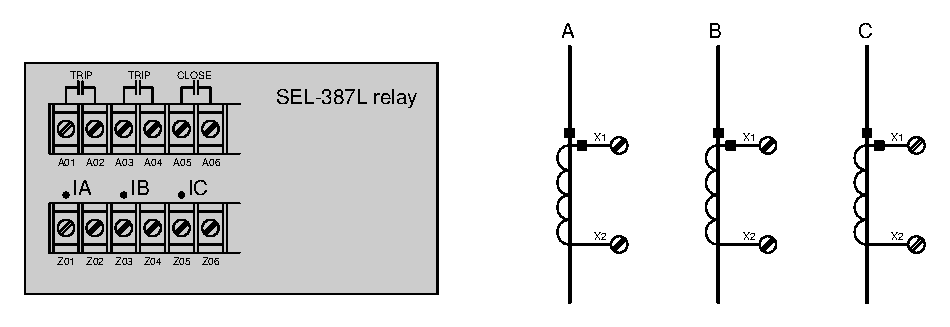
\includegraphics[width=15.5cm]{i03020x05.eps}$$

\vskip 20pt

\item{$(2)$} Explain what is meant by the labels {\tt 400:5} and {\tt C800} on a current transformer.

\vskip 20pt

\item{$(3)$} Calculate the phase voltage of a balanced 3-phase ``Wye'' load given a ``Delta'' source having a phase voltage of 2400 volts.  Also, calculate line current assuming each phase of the ``Wye'' load is a 50 ohm resistor.

\vskip 20pt

\filbreak

\item{$(4)$} Suppose the power transformer feeding the substation's east bus suffers an internal phase-to-ground fault in one of its primary windings.  Identify the {\it first} protective relay which should trip to protect the system from further damage.  Then, identify which circuit breaker(s) must trip in order to clear this transformer fault:

$$\includegraphics[width=15.5cm]{i03020x06.eps}$$

%INDEX% Lab exercise, motor control circuit (relay-based)

%(END_NOTES)


